\documentclass{standalone}

\usepackage{tikz}
\usetikzlibrary{shapes, arrows.meta, positioning}

\begin{document}
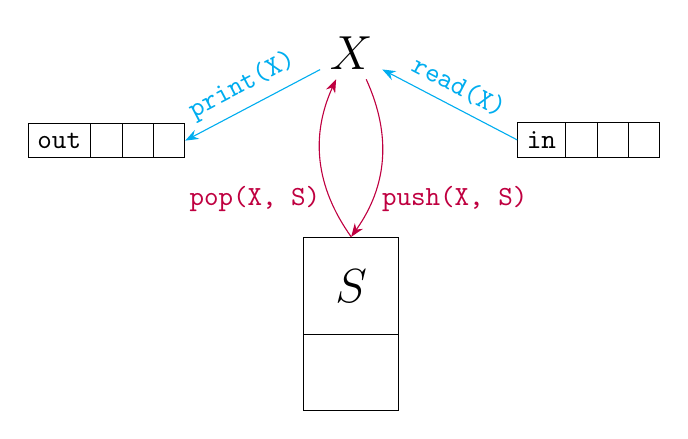
\begin{tikzpicture}[seq/.style = {rectangle split, 
  rectangle split horizontal, 
  rectangle split draw splits = true, 
  rectangle split parts = 4,
  draw}]

  \node[draw, rectangle split,
  	rectangle split parts = 2,
	inner sep = 4mm
      ] (stack) {\LARGE $S$};

  \node[seq, above right = 1.0cm and 1.5cm of stack] (in) {\texttt{in}};
  \node[seq, above left = 1.0cm and 1.5cm of stack] (out) {\texttt{out}};

  \node[above = 2.0cm of stack] (x) {\LARGE $X$};

  \draw[->, >=Stealth, cyan] (in.west) to node[sloped, above] {\texttt{read(X)}} (x);
  \draw[->, >=Stealth, cyan] (x) to node[sloped, above] {\texttt{print(X)}} (out.east);

  \draw[->, >=Stealth, bend left, purple] (x) to node[right, near end] {\texttt{push(X, S)}} (stack.north);
  \draw[->, >=Stealth, bend left, purple] (stack.north) to node[left, near start] {\texttt{pop(X, S)}} (x);
\end{tikzpicture}
\end{document}